\section{SB04 -- Protein Folding}

\subsection*{Table of Contents}
\begin{enumerate}
\item Protein folding problem
\item Native and denatured states
\item Levinthal's paradox
\item Secondary structure
\item Folding pathways
\item Energy landscape
\item Thermodynamics of folding
\item Folding kinetics
\item Chaperones
\item Misfolding and aggregation
\end{enumerate}

\subsection*{Possible questions:}
\begin{enumerate}
\item{\textcolor{blue}{What is the native state of a protein?}}
\item{What is the protein folding problem?}
\item{What is the typical folding timescale in biological proteins?}
\item{What is Levinthal's paradox?}
\item{What are the main secondary structures?}
\item {What are the backbone dihedral angles?}
\item {What is the Ramachandran plot?}
\item {How can we describe the folding process in terms variations of thermodynamic variables?}
\item{What is the hydrophobic effect?}
\item{What stabilizes the native state?}
\item{Difference between thermodynamics and kinetics of folding?}
\item{Why is protein folding not a random search?}
\item{Explain the energy funnel model.}
\item {What is the principle of minimal frustration?}
\item {What is residual frustration and why is it important?}
\item{What are molecular chaperones?}
\item{How is misfolding related to disease?}
\end{enumerate}

\newpage

\paragraph{What is the protein folding problem?}
Most proteins in biological systems are functional only when they are folded into a specific 3D structure, called the native state. The process by which a protein acquires its native structure is called folding. The protein folding problem is the challenge of understanding both \textbf{which} is the 3d structure that the protein will fold into (the native structure) starting from the sequence, and \textbf{how}
it will get there, meaning which sequence of conformations will it sample, and if there is a specific, dominant pathway that it will follow, or many.


So the protein folding problem has mainly two parts: one is the \textbf{structure prediction problem}, which is the question that methods like AlphFold are trying to answer,
and the other is the \textbf{folding mechanism problem}, which is the question of how the protein gets to its native state, and regards the kinetics of folding.

The structure prediction problem is framed like this: given the aminoacid sequence, find the \textbf{injective function} that maps the sequence to the 3D structure. 
Methods like alphafold try to learn this function from the data, and they are very successful at it. However, they do not give us any insight into the folding mechanism problem, which is still an open question.
Also, these methods are instrinsically limited by the data they are trained on: for instance, they only predict with a water environment, cannot say anything about what happens when the protein 
is in a different solvent, and they saw only the 20 L-aminoacids in the training data, so they cannot predict what happens when there are post-translational modifications, or non-natural aminoacids.


\paragraph{What is the typical folding timescale in biological proteins?}
Most biological proteins fold spontaneously on timescales ranging from microseconds to seconds, although the exact folding rate depends on protein size, topology, and stability. Small single-domain proteins can fold in microseconds or milliseconds, whereas larger proteins may require seconds or the assistance of molecular chaperones.


\paragraph{What is Levinthal's paradox?}

Levinthal's paradox is the observation that proteins fold into their native structure much faster than would be possible if they explored all possible conformations randomly. Cyrus Levinthal estimated that even a small protein could adopt an astronomically large number of conformations, making a random search of conformational space effectively impossible within the age of the universe.
However, experimental observations show that most proteins fold in times ranging from microseconds to seconds. This apparent contradiction suggests that protein folding is not a random search process. Instead, proteins fold through biased pathways guided by an energy landscape that directs the molecule toward the native state.
Additionally, biological proteins are not random sequences, but have been selected through evolution to fold in timescales compatible with life.

\paragraph{What are the main secondary structures?}
Secondary structure refers to local, regularly recurring arrangements of the protein backbone \textbf{stabilized primarily by hydrogen bonds} between backbone amide and carbonyl groups. The two most common secondary structures are the $\alpha$-helix and the $\beta$-sheet.
An $\alpha$-helix is a right-handed helical structure in which each carbonyl oxygen forms a hydrogen bond with the amide hydrogen four residues ahead in the sequence ($i \rightarrow i+4$). A $\beta$-sheet consists of extended $\beta$-strands connected by hydrogen bonds and can be either parallel or antiparallel. The antiparallel arrangement
is the most stable because it allows atoms that participate in the hydrogen bond to get closer.

\paragraph{What are the backbone dihedral angles?}
\begin{center}
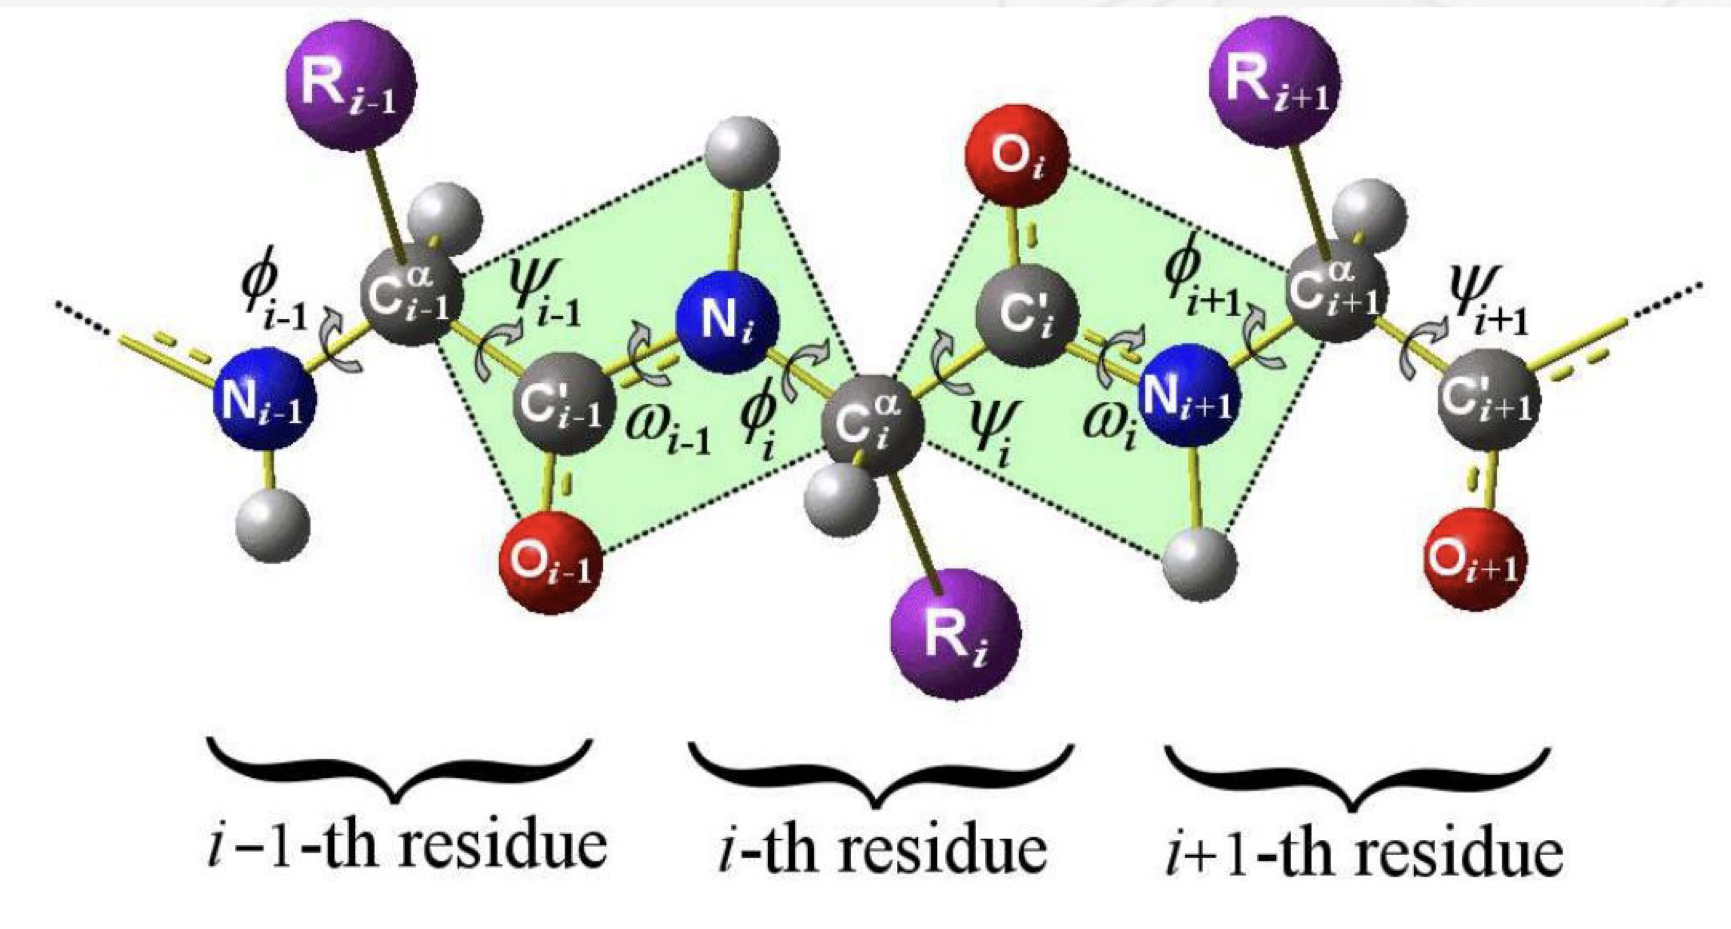
\includegraphics[width=0.5\textwidth]{figures/dihedrals.png}
\end{center}
The bond $N-C_\alpha - C_{\beta}$ is rigid and planar. Therefore, the backbone conformation of a protein can be described by two dihedral angles: $\phi$ (phi) and $\psi$ (psi). The $\phi$ angle is the rotation around the N-$C_\alpha$ bond and is defined by the three atoms ($C_{\beta}^{-1}, N,C_{\alpha}$), while the $\psi$ angle is the rotation around the $C_\alpha - C_{\beta}$ bond
and is defined by the three atoms ($C_{\alpha}, C_{\beta}, N^{+1}$). 

\paragraph{What is the Ramachandran plot?}
The Ramachandran plot is a graphical representation of the backbone dihedral angles $\phi$ and $\psi$ . Each point on the plot corresponds to a particular combination of these two angles, allowing visualization of the conformational space accessible to the protein backbone.
Because of steric repulsion between atoms, many combinations of $\phi$ and $\psi$ are energetically unfavorable and therefore forbidden. As a result, residues cluster in a few allowed regions corresponding to common secondary structures. For example, right-handed $\alpha$-helices and $\beta$-sheets occupy distinct areas of the Ramachandran plot.
The Ramachandran plot is widely used to understand protein structure and to assess the quality of experimentally determined or predicted structures. A high-quality protein model should have most residues located in energetically allowed regions, while residues in disallowed regions may indicate structural errors or unusual conformations.


\paragraph{How can we describe the folding process in terms of variations of thermodynamic variables?}

Protein folding can be described using the Gibbs free energy change

\[
\Delta G_{fold} = \Delta H_{fold} - T\Delta S_{fold}.
\]

Folding is thermodynamically favorable when $\Delta G_{fold}<0$, meaning that the folded state has a lower free energy than the unfolded state. The enthalpy term $\Delta H_{fold}$ is generally negative because folding creates stabilizing interactions such as hydrogen bonds, van der Waals contacts, and salt bridges.

The entropy change has two opposing contributions:

\[
\Delta S_{fold} = \Delta S_{conf} + \Delta S_{solvent}
\]

The protein loses conformational freedom upon folding, leading to a decrease in conformational entropy ($\Delta S_{conf}<0$), which opposes folding. However, hydrophobic residues become buried in the protein core, releasing ordered water molecules into the solvent and increasing solvent entropy ($\Delta S_{solvent}>0$), which favors folding.

Overall, the sign of $\Delta G_{fold}$ depends on the balance between these enthalpic and entropic contributions. Usually it is negative, meaning that the folded state is thermodynamically favored. But not by a lot: it is said that proteins are "marginally stable": the free energy difference between the folded and unfolded states is typically only a few kcal/mol ($5-15$), which is 
small compared to the total energy of the protein (for a comparison, a single hydrogen bond acocunts for $1-5\, kcal/mol$). This marginal stability allows proteins to be flexible and dynamic, enabling them to perform their biological functions effectively.


\paragraph{What is the hydrophobic effect?}
The hydrophobic effect is the tendency of nonpolar molecules or side chains to cluster together in aqueous environments. In proteins, hydrophobic residues such as Val, Leu, Ile, Phe, and Met are typically buried in the protein core, while polar and charged residues remain exposed to the solvent.
The driving force behind the hydrophobic effect is not a direct attraction between hydrophobic groups. Instead, it arises from the behavior of water molecules. When hydrophobic residues are exposed, surrounding water molecules become highly ordered to maintain their hydrogen-bonding network. This ordering decreases the entropy of the solvent. Upon folding, hydrophobic residues are buried, reducing the exposed hydrophobic surface and releasing these ordered water molecules into the bulk solvent, thereby increasing solvent entropy.
The hydrophobic effect is one of the major driving forces of protein folding. 


\paragraph{Why is protein folding not a random search?}
Because it cannot be. The Levital's paradox assumed that every residue can sample all possible conformations independently. But this is not true, there are constraints on the conformational space that the protein can sample, such as steric hindrance and the formation of local secondary structures. These constraints significantly reduce the number of conformations that need to be explored.
Also, the folding process is guided by an energy landscape that directs the protein towards the native state. As some of the native interaction form, the space of possibilities gets restricted and 
other native interactions become more likely to form, and this goes on till the protein reaches the minimum of the energy landscape, which is the native state. 





\paragraph{Explain the energy funnel model view and how it differs from the ant trail view}
The funnel model essentially says that at the start of the folding process, the protein can sample a wide variety of conformations, but as it folds and forms native interactions, the conformational space narrows down. 
This is a funnel-shaped energy landscape, where the bottom represents the native state. The folding process is stochastic: usually there is no "single" pathway dominating over the others.
Different molecules of the same protein may follow different routes and visit different intermediates, yet still reach the same native structure.



\paragraph{What is the principle of minimal frustration?}

Frustration means that different interactions “disagree” about what the structure should be. Minimal frustration means that most interactions “agree” that the native state is the best solution.
This concept is tightly connected to the energy funnel model: the funnel exists precisely because evolution has minimized frustration in naturally occurring protein sequences.


The principle of minimal frustration states that natural proteins have evolved sequences in which most interactions favor the formation of the native structure rather than competing with it. As a result, the energy landscape is biased toward the native state and contains relatively few energetic conflicts, or \emph{frustrations}, that could trap the protein in incorrect conformations. It is
overall a quite smooth landscape. This greatly reduces the number of kinetic traps and allows proteins to fold rapidly and reproducibly.


\paragraph{What is residual frustration and why is it important?}

Although natural proteins obey the principle of minimal frustration, frustration is not completely eliminated. \emph{Residual frustration} refers to the small number of interactions within a folded protein that are not fully optimized for structural stability and that locally favor alternative conformations or competing interactions.
Residual frustration is important because proteins are not evolved solely for stability. Many functional processes, such as ligand binding, allosteric regulation, conformational changes, and enzymatic catalysis, require a certain degree of flexibility and structural adaptability. Locally frustrated regions often coincide with active sites, binding interfaces, or regions involved in molecular recognition.
Therefore, while minimal frustration enables efficient folding by creating a funnel-shaped energy landscape, residual frustration provides the flexibility necessary for biological function. Proteins can be viewed as a compromise between the requirements of stability and the requirements of activity.

\paragraph{How is misfolding related to disease?}

Protein misfolding occurs when a protein fails to reach its native structure or adopts an alternative conformation that is unstable or non-functional. Misfolded proteins may lose their biological activity, become degraded, or aggregate with other misfolded molecules. Because protein function depends strongly on structure, misfolding can have severe cellular consequences.
Many diseases are associated with the accumulation of misfolded proteins and the formation of insoluble aggregates or amyloid fibrils. Examples include Alzheimer's disease, which involves aggregation of amyloid-$\beta$ peptides; Parkinson's disease, associated with $\alpha$-synuclein aggregates; and prion diseases, in which a misfolded protein induces the misfolding of other copies of the same protein. In these cases, protein aggregation can disrupt cellular processes and lead to cell death.
Cells possess quality-control mechanisms, including molecular chaperones and degradation pathways, that help proteins fold correctly and remove misfolded species. Disease can arise when these systems are overwhelmed or when mutations increase the tendency of a protein to misfold and aggregate.